\documentclass[12pt]{article}

\usepackage{fullpage}
\usepackage{multicol, multirow}
\usepackage{tabularx}
\usepackage{standalone}
\usepackage{listings}
\usepackage{ulem}
\usepackage{amsmath}
\usepackage{pdfpages}
\usepackage[utf8]{inputenc}
\usepackage[russian]{babel}

\newcommand{\StudentName}{Ильвохин Дмитрий}
\newcommand{\Group}{1O-106М}
\newcommand{\CourseName}{Программирование игр}
\newcommand{\LabNum}{1}
\newcommand{\Subject}{Воздушная битва}
\newcommand{\PrepName}{Аносова Н.\,П.}

\begin{document}

\documentclass[a4paper, 12pt]{report}
\usepackage[english, russian]{babel}
\usepackage[utf8]{inputenc}
\usepackage{amssymb, amsfonts, amsmath, mathtext, cite, enumerate, float}
\usepackage{geometry}
\usepackage{chngpage}

\begin{document}

\begin{titlepage}

\newpage

\begin{center}
Московский Авиационный Институт \\*
(национальный исследовательский университет) \\*
Факультет прикладной математики и физики \\*
\hrulefill
\end{center}

\begin{center}
Кафедра вычислительной математики и программирования
\end{center}

\vspace{6em}

\begin{center}
\Large \CourseName \\
	Курсоваой проект \\
  <<\Subject>>
\end{center}

\vspace{2em}
\vspace{6em}

\begin{flushright}
	\StudentName, \\
	группа: \Group \\
\vspace{1em}
преподаватель:\\
   \PrepName \\
\end{flushright}

\vspace{\fill}

\begin{center}
Москва, 2015
\end{center}

\end{titlepage}

\end{document}
 % title page

\lstset
{
        language=Python,
        basicstyle=\footnotesize,% basic font setting
        extendedchars=\true
}

\subsection*{Задание}

Разработать законченную 2D или 3D игру.

\subsection*{Практическая часть}
Для реализации игры был выбран движок LÖVE (love2d) --- свободно распространяемый игровой движок,
предназначенный для написания компьютерных игр на языке Lua.

В отличие от многих популярных движков LÖVE не представляет и себя конструктор игр.
Для написания кода игры можно использовать любой текстовый редактор с подсветкой синтаксиса языка Lua.
Также в нём нет редактора уровней, все изображения, уровни и персонажи прописываются в коде игры.~\cite{love}

\begin{figure}[!htb]
  \centering
    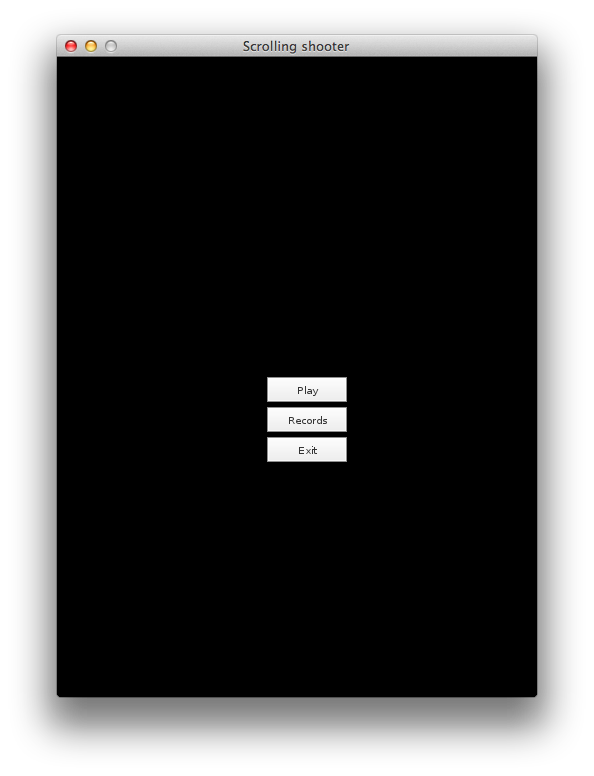
\includegraphics[scale=0.5]{pics/start.png}
   \caption{Стартовое меню}
    \label{fig:start}
\end{figure}

\begin{figure}[!htb]
  \centering
    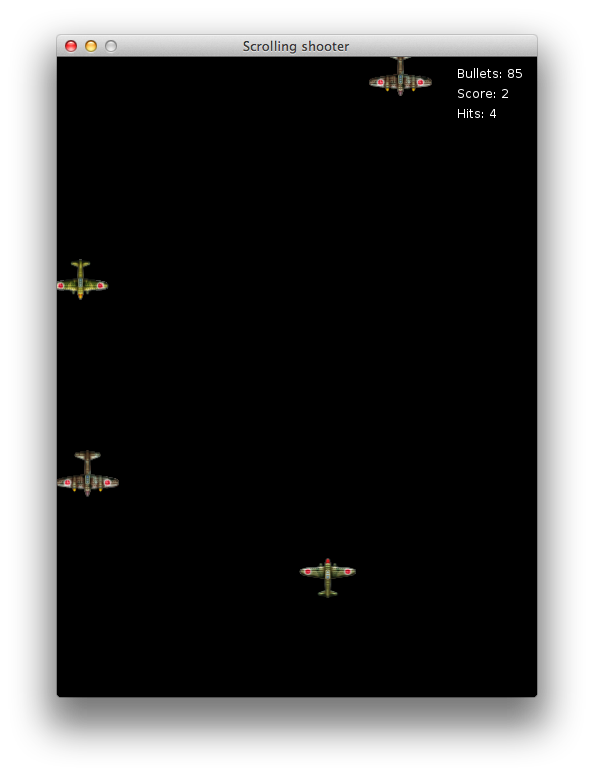
\includegraphics[scale=0.5]{pics/game.png}
   \caption{Скриншот игры}
    \label{fig:game}
\end{figure}

\begin{figure}[!htb]
  \centering
    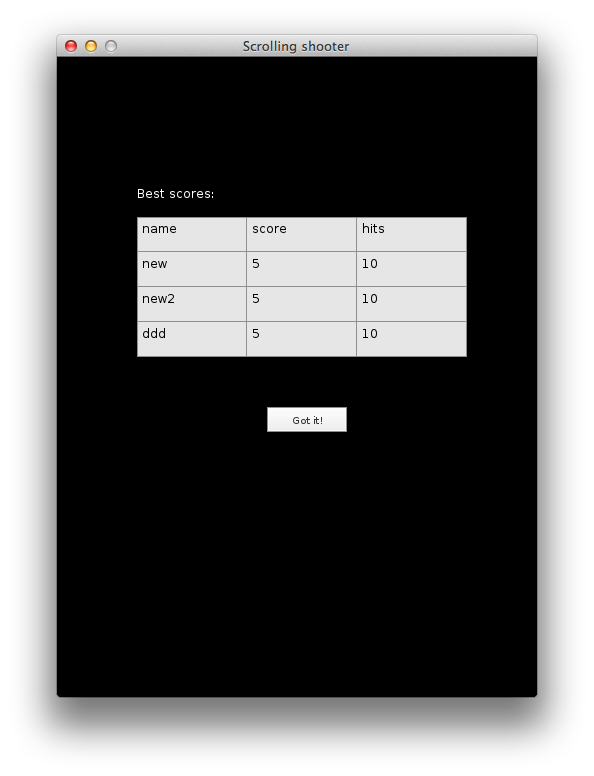
\includegraphics[scale=0.5]{pics/records.png}
   \caption{Таблица рекордов}
    \label{fig:start}
\end{figure}

\subsection*{Выводы}

\begin{thebibliography}{}
\bibitem{love} https://ru.wikipedia.org/wiki/LÖVE
\bibitem{love_official} https://love2d.org/wiki/Main\_Page
\end{thebibliography}

\end{document}

